\chapter{Introduction to Quantum Computing} \label{chap:introduction}

In recent years, new and promising computing paradigms and architectures have emerged, complementing (and possibly competing with or outperforming in the near future) classical computing to solve highly complex problems. Among them, quantum computing stands out as one of the most promising and disruptive paradigms, expected to fundamentally revolutionize the way we process information. 

This paradigm is profoundly different from classical computing, which uses a binary system of bits (0 or 1) to represent and process data. Quantum computing harnesses qubits, a completely different representation of information. Through quantum superposition, a qubit can exist simultaneously in a combination of states $|0\rangle$ and $|1\rangle$. Furthermore, quantum entanglement allows a deep correlation between qubits even over large distances, enabling the system to represent and process information in a fundamentally different way, with the potential to outperform classical computing in specific tasks \cite{quantumReport, nielsen2010quantum}.

In this chapter, we will provide a brief overview of quantum computing, its evolution, and its promises. We will also compare different hardware paradigms, focusing on superconductors and neutral atoms, and discuss the characteristics and geometric constraints of neutral atom platforms.

\section{Promises of quantum computing}
\label{sec:evolution_promises}

The quantum computing paradigm currently promises to revolutionize information processing, offering the potential to solve problems that are intractable for classical computers. It is thus immediate to consider all the potential applications and fields that are currently facing the computational limits of NP-hard problems. While many heuristics, approximation algorithms, and metaheuristics have been developed to solve these problems, they are not always able to provide optimal solutions. Consequently, it is straightforward to recognize the potential of quantum computing in fields such as cryptography, optimization, machine learning, and drug discovery \cite{memon2024quantum}, where the ability to process large datasets and solve NP-hard problems on larger scales can lead to significant breakthroughs. 

A comprehensive overview of the main promises of quantum computing (and neutral atoms in particular) can be found in \cite{grotti2026practicalusecasesneutral}, which discusses the primary characteristics and potential use cases of this technology. Additionally, a complete panorama of this paradigm, including its challenges, is detailed in \cite{quantumReport}. Finally, to provide a summarized but complete introduction, we can conclude that quantum computing is a disruptive paradigm offering new opportunities for solving complex problems in various fields. However, it is still in its early stages of development, and many challenges remain to be addressed before it can reach its full potential.

These limitations and challenges must not be seen as a reason to avoid exploring this paradigm, but rather as a motivation to understand its boundaries and develop new algorithms capable of leveraging its unique capabilities. The importance of this matter is highlighted by the sector's market capitalization, estimated at approximately USD 10.13 billion in 2022 and projected to reach USD 125 billion by 2030 \cite{quantumReport}.

In the following sections, the main characteristics of neutral atom quantum computing are explored in more detail, together with their physical constraints, to provide a clear sense of why our exploration will face specific limitations in the next chapters of this thesis.

\section{Hardware paradigms compared: Superconductors vs. Neutral Atoms}
\label{sec:hardware_paradigms}

Currently, the quantum computing landscape is characterized by rapid technological advancement and intense competition. A diverse ecosystem of tech giants, research institutions, and startups is actively investigating various physical architectures. The shared objective is to develop a highly efficient and scalable computing paradigm capable of overcoming the fundamental challenges of the field, primarily quantum noise, limited coherence times, and hardware scalability \cite{quantumReport}.

To illustrate the diversity of this ecosystem, it is sufficient to look at the different technological pathways chosen by major industry players. Companies such as Google \cite{google2024whatisquantum}, Microsoft \cite{microsoft_majorana1}, and D-Wave \cite{mcgeoch2020dwaveReview} have heavily invested in superconducting qubits, whereas startups like Pasqal \cite{Henriet2020quantumcomputing} and QuEra Computing \cite{ebadi2022quantum} are pioneering platforms based on neutral atoms. Simultaneously, other organizations are exploring alternative technologies, including trapped ions, photonic circuits, silicon spin qubits, and innovative quantum error correction approaches, such as the hardware-efficient \textit{cat qubits} developed by Alice \& Bob \cite{alicebob2024white}, which aim to intrinsically mitigate decoherence and pave the way toward fault-tolerant architectures.

This section provides a comparative analysis of the two most prominent paradigms relevant to this work: superconducting circuits and neutral atoms.

\subsection{Superconducting qubits}

Without delving deeply into the physical details (which are beyond the scope of this thesis), superconducting qubits are based on Josephson junctions, superconducting circuits that exhibit quantum behavior at temperatures near absolute zero. These qubits are typically fabricated using advanced lithographic techniques and can be integrated into complex solid-state circuits. Superconducting qubits offer the advantage of very fast gate operations and relatively high fidelity, but they require extreme cryogenic cooling to maintain their quantum state \cite{google2024whatisquantum}. 

A comprehensive overview of superconducting qubit technologies and the major players leading the field can be found in \cite{memon2024quantum}. Currently, this type of qubit is the most mature and widely adopted in the industry; nevertheless, it faces significant challenges regarding scalability and coherence times. The strict requirement for cryogenic cooling and the engineering complexity of scaling up the number of qubits while maintaining high fidelity and mitigating cross-talk remain significant obstacles to achieving practical, large-scale quantum computing \cite{memon2024quantum}.

D-Wave is among the most well-known companies in this space, having developed commercial quantum annealers based on superconducting qubits designed specifically to solve optimization problems \cite{mcgeoch2020dwaveReview}. It is important to note that D-Wave's approach differs from the universal gate-based model pursued by Google and IBM, as it is tailored for specific optimization landscapes rather than general-purpose computing. However, for Quadratic Unconstrained Binary Optimization (QUBO) problems (which represent the core mathematical framework investigated in this thesis) quantum annealing remains one of the most effective approaches. While D-Wave's specific platform will not be extensively discussed in the remainder of this work, it stands as a commercially viable benchmark for solving large QUBO instances through purely quantum or hybrid approaches.

\subsection{Neutral Atom platforms}

Neutral atom platforms, on the other hand, utilize individual atoms trapped in optical lattices or optical tweezers to act as qubits. These atoms can be manipulated using finely tuned laser light, allowing their quantum states to be controlled with extreme precision. A primary advantage of neutral atom systems is their excellent isolation from the environment, which translates into long coherence times. Furthermore, they offer significant scalability potential, as large arrays of atoms can be trapped, dynamically positioned, and manipulated simultaneously. However, they also face significant engineering challenges, particularly regarding the complexity of controlling massive optical arrays and maintaining atomic stability within the traps over extended periods \cite{Henriet2020quantumcomputing, memon2024quantum}.

These platforms are exceptionally promising for quantum simulation and combinatorial optimization tasks. By exciting the atoms to highly energetic states, they can naturally implement strong, long-range interactions that are difficult to achieve natively with other qubit technologies \cite{Henriet2020quantumcomputing}. Due to this inherent physical capability, neutral atom architectures represent the primary focus of this thesis. 

Among the main players in the field, Pasqal and QuEra Computing are notable for their pioneering work in developing these platforms. These companies have made significant strides in demonstrating the feasibility of large-scale neutral atom systems and their potential applicability in solving complex optimization problems \cite{ebadi2022quantum, Henriet2020quantumcomputing, memon2024quantum}.

Specifically, this work explores a hybrid quantum-classical architecture designed to tackle large-scale QUBO problems using these precise devices. Consequently, their capabilities and constraints are extensively investigated and discussed throughout the following chapters. As a foundation, the next section details the main characteristics and geometric constraints inherent to neutral atom platforms, which act as crucial parameters for the design of the hybrid architecture proposed in this thesis.

\section{Characteristics of Neutral Atom platforms}
\label{sec:neutral_atoms_constraints}

This section focuses on the main characteristics and geometric constraints of neutral atom platforms, which are crucial for understanding the limitations and capabilities of these systems in the context of solving large-scale QUBO problems.

\paragraph{Neutral atom arrays}

A neutral atom array can be conceptualized as a hardware register where each individual atom acts as a qubit. These atoms are arranged in 1D, 2D (as in the context of this work), or 3D configurations \cite{Henriet2020quantumcomputing, Vercellino_2022}, as illustrated in Figure \ref{fig:neutral_arrays}.

\begin{figure}[htbp]
    \centering
    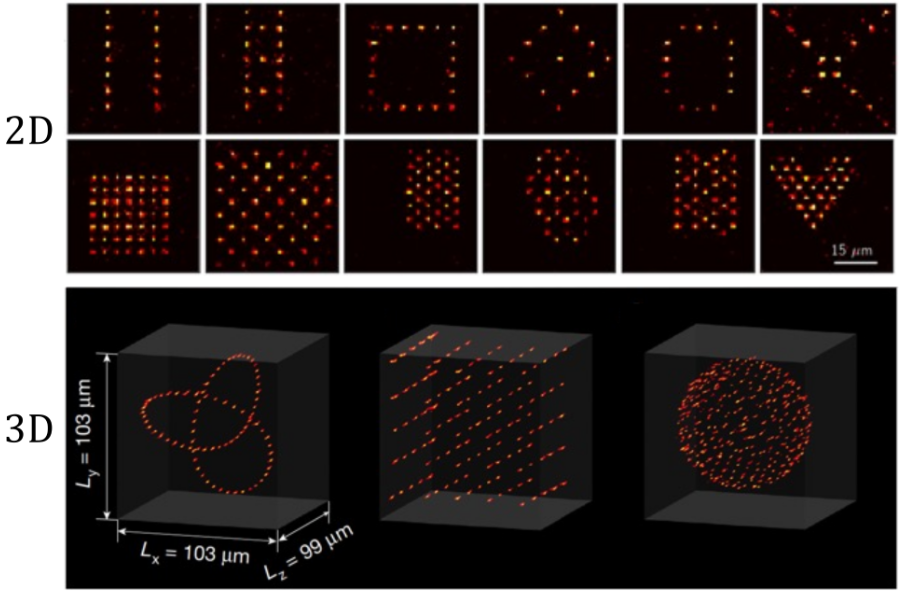
\includegraphics[width=0.8\textwidth]{img/2D-3D_neutral_atom_reg.png}
    \caption{2D and 3D neutral atom arrays. Image extracted from \cite{Henriet2020quantumcomputing}.}
    \label{fig:neutral_arrays}
\end{figure}

Unlike superconducting systems, where qubits are statically fabricated on a physical chip, neutral atoms can be dynamically arranged and manipulated using optical tweezers. This inherent flexibility allows for the creation of custom geometries and the implementation of specific interaction topologies between qubits, which is highly advantageous for solving optimization problems that demand tailored connectivity.

However, because the register is not permanently fixed, it must be reconstructed for each computation cycle. The overall execution process consists of three main phases:
\begin{itemize}
    \item Register preparation
    \item Quantum processing
    \item Register readout
\end{itemize}

The primary focus of this thesis, however, precedes the physical execution phase. It centers on the algorithmic challenge of efficiently embedding a QUBO problem onto this spatially constrained register to find optimal or near-optimal solutions. While the remainder of this work focuses mainly on the algorithmic approach, leveraging libraries and remote simulation infrastructures rather than delving into low-level hardware control, understanding the physical constraints of the QPU is essential. Therefore, following the explanations provided by \cite{Henriet2020quantumcomputing}, we briefly outline the physical mechanisms behind register loading and readout.

\paragraph{Register loading}
Configuring the atomic register requires a complex optical setup, relying on arrays of optical tweezers alongside the components illustrated in Figure \ref{fig:qpu_components}.

\begin{figure}[htbp]
    \centering
    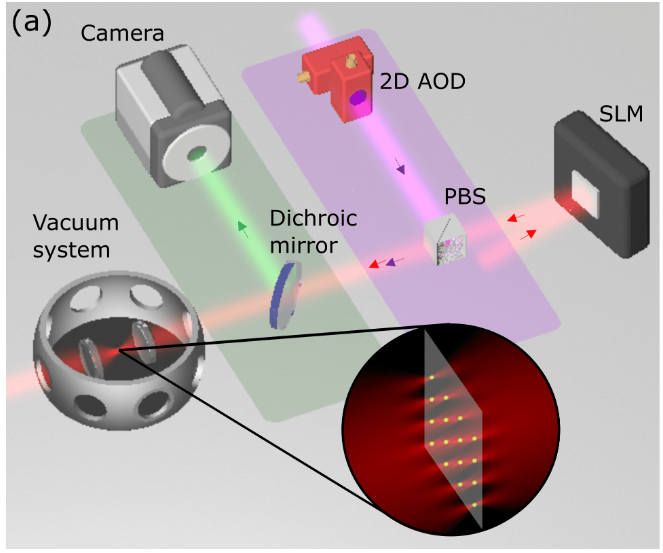
\includegraphics[width=0.8\textwidth]{img/principal_compo_QPU.png}
    \caption{Main hardware components of a neutral atom QPU. The trapping laser light (red) is shaped by a Spatial Light Modulator (SLM). Moving tweezers (purple), used to rearrange atoms, are controlled by a 2D Acousto-Optic Deflector (AOD) and superimposed using a Polarizing Beam-Splitter (PBS). The green fluorescence emitted by the atoms is separated by a dichroic mirror and captured by a camera during the readout phase. Image adapted from \cite{Henriet2020quantumcomputing}.}
    \label{fig:qpu_components}
\end{figure}

In essence, the process begins inside a vacuum chamber, where a laser system cools and confines a cloud of atoms. Subsequently, high-precision lenses focus light beams into extremely tight spots, creating optical tweezers. Each optical trap is designed to isolate and hold a single atom. By leveraging holographic techniques through a Spatial Light Modulator (SLM), it is possible to project these tweezers into predefined positions, generating the desired geometric array. This mechanism is the cornerstone of the technology's scalability: theoretically, scaling the system primarily requires increasing laser power and improving optical resolution to project more traps.

However, loading atoms from the cooled cloud into the traps is a stochastic process. Due to light-assisted collisions, each optical tweezer has roughly a 50\% probability of capturing exactly one atom, leaving the remaining traps empty. To construct a defect-free computational register, the system must perform an active rearrangement. This is achieved using dynamic tweezers governed by Acousto-Optic Deflectors (AODs), which sort and move atoms from filled traps into empty ones. This sorting process is repeated until the target array is completely filled, resulting in a perfect register ready for the quantum processing phase \cite{Henriet2020quantumcomputing}.

\paragraph{Quantum processing and register readout}

Once the atomic array is perfectly assembled, the quantum processing phase can begin. It is worth noting a significant timescale disparity in this hardware: while the actual quantum computation (performed via precisely timed laser pulses) is extremely fast, typically lasting less than 100 \textmu s, the entire computational cycle is dominated by the physical loading and readout phases, requiring approximately 200 ms in total \cite{Henriet2020quantumcomputing}.

After the algorithm is executed, the final state of the register must be measured to extract the classical solution. This readout phase is performed through fluorescence imaging. The physical system is tuned so that atoms remaining in the ground state (representing the logical qubit state $|0\rangle$) emit photons and appear as bright spots on the image. Conversely, atoms excited to the Rydberg state (representing the logical qubit state $|1\rangle$) do not fluoresce and remain dark. 

These optical signals are captured by highly sensitive Electron-Multiplying CCD (EMCCD) cameras. This detection method is extremely reliable, reaching readout efficiencies above 98.6\%, a performance highly competitive with the readout fidelities typical of superconducting circuits \cite{Henriet2020quantumcomputing}. Finally, due to the inherently probabilistic nature of quantum mechanics, a single execution yields only one possible classical bit-string. Therefore, the complete sequence of preparation, processing, and readout must be repeated hundreds or thousands of times (taking multiple \textit{shots}) to reconstruct the statistical probability distribution of the outcomes and successfully identify the optimal solution.

\paragraph{Quantum analog mode execution}

Neutral atom platforms can operate in both digital and analog modes. This work concentrates exclusively on the latter; please refer to \cite{Henriet2020quantumcomputing} for more information on the former. The dynamics of the analog mode are well-described by the Ising model, governed by the following Hamiltonian:

\begin{equation}
    \hat{\mathcal{H}}(t)=\hbar\sum_{i=1}^{N}\left(\frac{\Omega(t)}{2}\hat{\sigma}_{i}^{x}-\delta(t)\hat{n}_{i}\right)+\sum_{i<j}\frac{C_{6}}{|r_{i}-r_{j}|^{6}}\hat{n}_{i}\hat{n}_{j}
\end{equation}

This equation can be conceptually divided into two parts. The first summation dictates the evolution of single atoms driven by the external laser field, while the second summation governs the interactions between pairs of atoms. Specifically, the parameters and operators are defined as follows:
\begin{itemize}
    \item $N$ is the total number of atoms (qubits) in the register;
    \item $\Omega(t)$ is the time-dependent Rabi frequency, representing the amplitude of the laser exciting the atoms;
    \item $\delta(t)$ is the detuning parameter of the laser frequency;
    \item $\hat{\sigma}_{i}^{x}$ is the Pauli-X operator acting on atom $i$, which drives the transition between the ground state $|0\rangle$ and the Rydberg state $|1\rangle$;
    \item $\hat{n}_{i}$ is the occupation number operator (defined as $|1\rangle_i\langle 1|_i$) which evaluates to 1 if atom $i$ is in the Rydberg state, and 0 otherwise;
    \item $r_i$ is the spatial position of atom $i$;
    \item $C_6$ is the Van der Waals interaction coefficient, which is a constant dependent on the specific atomic species and platform used \cite{nowak2026satellitemissionplanningrydberg}.
\end{itemize}

Crucially, the third term in this Hamiltonian represents the interaction between individual spins. It accounts for the energy penalty incurred when two spatially close qubits occupy the Rydberg state simultaneously. When excited, qubits transition to the Rydberg state; however, if they are physically in close proximity, they experience the \textit{Rydberg blockade effect}. In this regime, maintaining the Rydberg state by the first qubit heavily suppresses the excitation of the second. Qubits in Rydberg states interact with each other proportionally to the third term above, following the Van der Waals potential for dipole-dipole interactions:

\begin{equation}
V_{ij} = \frac{C_6}{r_{ij}^6}
\end{equation}

where:
\begin{itemize}
    \item $V_{ij}$ is the interaction energy between atoms $i$ and $j$;
    \item $C_6$ is the Van der Waals coefficient, which depends on the atom type and scales massively with the excitation level;
    \item $r_{ij}$ is the spatial distance between the two atoms \cite{Henriet2020quantumcomputing}.
\end{itemize}